\section{Vægtede grafer}

Flere problemstillinger kan modelleres ved brug af grafer med vægte tildelt kanterne. 
Det kan f.eks. være distance, den samlede rejsetid, eller billetprisen for at rejse mellem to byer. 
Grafer, der har vægte tildelt kanterne, kaldes vægtede grafer. 
Der opstår jævnligt forskellige typer af problemer, der involverer vægtede grafer, hvor en korteste rute, mellem to knuder i et netværk, skal bestemmes. 
Længden af en vej i en graf uden vægte er tidligere betegnet ved antallet af kanter, vejen går igennem.
I en vægtet graf er længden af vejen summen af alle kanternes vægte, der indgår i vejen. \\
I Figur \ref{fig:weighted_graph} ses et eksempel på en vægtet graf. Den kortest mulige vej fra $A$ til $D$ må være $\lbrace A,C \rbrace$, $\lbrace C,E \rbrace$, $\lbrace E,F \rbrace$, $\lbrace F,D \rbrace$. Denne vej har en længde på $5+5+5+5=20$. 

\begin{figure}[h!]
	\centering
	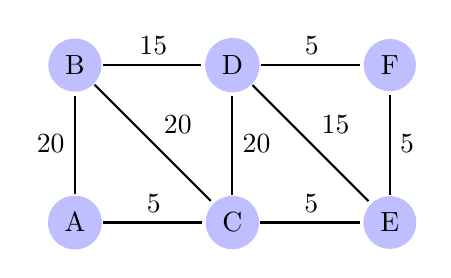
\begin{tikzpicture}[shorten >=1pt,auto,node distance=2cm,thick,main node/.style={circle,fill=blue!25}]                      
  \node[main node] (F) {F};                
  \node[main node] (D) [left of=F] {D};    
  \node[main node] (E) [below of=F] {E};   
  \node[main node] (B) [left of=D] {B};    
  \node[main node] (C) [below of=D] {C};   
  \node[main node] (A) [below of=B] {A};   
              
	\path[-, draw, thick]
  (A) edge node {$20$} (B)
	(B) edge node {$20$} (C)
	(B) edge node {$15$} (D)
	(C) edge node[right] {$20$} (D)
	(C) edge node {$5$} (E)
	(D) edge node {$15$} (E)
	(D) edge node {$5$} (F)
	(E) edge node[right] {$5$} (F)
	(A) edge node {$5$} (C)
	;
\end{tikzpicture}

	\caption{Eksempel på en vægtet graf.} \label{fig:weighted_graph}
\end{figure}

Et interessant problem, som involverer vægtede grafer, søger en kreds af kortest mulig totallængde, der besøger hver knude i en komplet graf præcis én gang.

I Figur \ref{fig:weighted_graph} vil en kreds af kortest mulig længde være $\lbrace A,C \rbrace$, $\lbrace C,E \rbrace$, $\lbrace E,F \rbrace$, $\lbrace F,D \rbrace$, $\lbrace D,B \rbrace$, $\lbrace B,A \rbrace$.
Denne kreds har en længde på $5+5+5+5+15+20=55$.

Der er her tale om et eksempel på \emph{traveling salesperson problem}, som søger dén rækkefølge, knuderne skal besøges i, som resulterer i en kreds af kortest mulig længde. 
Dette problem vil projektet undersøge nærmere i et senere kapitel.

\subsection{En korteste-vej algoritme}
Der er flere algoritmer, som finder den korteste vej mellem to knuder i en vægtet graf.
Et eksempel på en sådan algoritme er Dijkstras algoritme.
Algoritmen bruges til at finde den korteste vej fra $a$ til $z$ (eller en hvilken som helst anden knude) for ikke-orienterede vægtede grafer, hvor alle vægte er positive, og kan let tilpasses orienterede grafer også.

Algoritmen bygger på en serie af gentagelser, hvor et sæt af knuder konstrueres, ved at tilføje én knude ved hver gentagelse. 
En knude $w$ bliver tildelt værdien (længden) af den korteste vej fra $a$ til $w$, der kun indeholder de knuder, der allerede er i sættet. 
Den knude, der tilføjes sættet, har den mindste værdi af de knuder, der allerede er en del af sættet.

Dijkstras algoritme starter ved at tildele $a$ værdien $0$ og de andre knuder med $\infty$. 
Der bruges notationerne $L_0(a)=0$ og $L_0(v)= \infty$ for disse, hvor $0$’et angiver, at det er den $0$te gentagelse. 
Disse værdier angiver længden af den korteste vej fra $a$ til de givne knuder, hvor vejen kun indeholder $a$. 
Der findes ingen vej fra $a$ til en knude forskellig fra $a$, hvorfor $\infty$ er længden af den korteste vej fra $a$ til en sådan knude.
Algoritmen fortsætter ved at forme et sæt af knuder. Sættet betegnes $S_k$ efter $k$ gentagelser. 
Til at begynde med er $S_0=\emptyset$. 
Sættet $S_k$ laves fra $S_(k-1)$ ved at tilføje en knude $u$ (med den mindste værdi), som ikke er i $S_(k-1)$.
Herefter opdateres værdierne af alle knuder, som ikke er i $S_k$, således $L_k(v)$ er længden af den korteste vej fra $a$ til $v$, som kun indeholder knuder i $S_k$. 
Den måde, hvorpå algoritmen vælger en knude $u$, der tilføjes $S_k$ ved hver gentagelse, er det optimale valg af knude, hvilket gør den til en grådig algoritme. 
Proceduren fortsætter med at tilføje knuder til sættet, indtil $z$ også er tilføjet.
Herefter tildeles $z$ den værdi, der svarer til længden af den korteste vej fra $a$ til $z$.

Dijkstras algoritme ses i Algoritme \ref{dijkstras_algorithm}.

\begin{algorithm}[!h]
	\caption{Dijkstras algoritme}
	\label{dijkstras_algorithm}
	\textbf{procedure} $Dijkstra(G:$ vægtet sammenhængende simpel graf, med positive vægte) \\ 
	$\lbrace G$ har knuder $a=v_0, v_1, \dotsc , v_n=z$ og længder $w(v_i,v_j)$ hvor $w(v_i,v_j)= \infty $ hvis $ \lbrace v_i,v_j \rbrace $ ikke er en kant i $G \rbrace$ \\
	\textbf{for} $i:=1$ \textbf{til} $n$ \\
	$\-$ $\-$ $\-$ $\-$ $\-$ $\-$
	$L(v_i):= \infty$ \\
	$L(a):=0$ \\
	$S:=\emptyset$ \\
	{værdien er nu fastsat, så værdien af $a$ er $0$ og alle andre værdier er $\infty$, og $S$ er et tomt sæt} \\
	$\-$ $\-$ $\-$ $\-$ $\-$ $\-$
	\textbf{så længe} $z \not\in S$ \\
	$\-$ $\-$ $\-$ $\-$ $\-$ $\-$
	$u:=a$ en knude $\not\in S$ med $L(u)$ minimum \\
	$\-$ $\-$ $\-$ $\-$ $\-$ $\-$
	$S:_S\cup \lbrace u \rbrace$ \\
	$\-$ $\-$ $\-$ $\-$ $\-$ $\-$
	\textbf{for} alle knuder $v \not\in S$ \\
	$\-$ $\-$ $\-$ $\-$ $\-$ $\-$
	$\-$ $\-$ $\-$ $\-$ $\-$ $\-$
	\textbf{hvis} $L(u)+w(u,v)<L(v)$ \textbf{så} $L(v):=L(u)+w(u,v)$ \\
	$\-$ $\-$ $\-$ $\-$ $\-$ $\-$
	$\-$ $\-$ $\-$ $\-$ $\-$ $\-$
	{dette tilføjer en knude til $S$ med minimal værdi og opdaterer værdien af knuderne $\not\in S$} \\
	\textbf{returner} $L(z)$ {$L(z)=$ længden af den korteste vej fra $a$ til $z$}
\end{algorithm} 

Til at opsummere dette opstilles Sætning \ref{dijkstras_theorem}.

\begin{thm}\label{dijkstras_theorem}
	Dijkstras algoritme finder længden af en korteste vej mellem to knuder i en sammenhængende, simpel, ikke-orienteret vægtet graf.
\end{thm}

\begin{proof}
	Den induktive hypotese gælder for den $k$te gentagelse. 
	Lad $v$ være knuden tilføjet til $S$ ved den $(k+1)$te gentagelse, så $v$ er en knude $\not\in$ $S$ i slutningen af den $k$te gentagelse med den mindste værdi (hvis der er flere knuder af samme værdi, vælges blot én af disse). \\
	Fra den induktive hypotese ses der, at knuderne i $S$ før den $(k+1)$te gentagelse er angivet med længden af den korteste vej fra $a$. 
	Så er $v$ angivet med længden af den korteste vej fra $v$ til $a$. 
	Hvis det ikke var tilfældet i slutningen af den $k$te gentagelse, ville der være en vej kortere end $L_k(v)$, der indeholder en knude $\not\in$ $S$. 
	Lad $u$ være den første knude $\not\in$ $S$ i sådan en vej. 
	Der er en vej med længder kortere end $L_k(v)$ fra $a$ til $u$ kun indeholdende knuder i $S$. 
	Dette modsiger valget af $v$, da $(i)$ holdes i slutningen af den $(k+1)$te gentagelse.
	Lad $u$ være en knude $\not\in$ $S$ efter $k+1$ gentagelser. 
	En korteste vej fra $a$ til $u$, som kun indeholder elementer i $S$, indeholder enten $v$ eller ikke. 
	Hvis den ikke indeholder $v$, er længden $L_k(u)$ ved den induktive hypotese. 
	Hvis den derimod indeholder $v$, må der laves en vej fra $a$ til $v$ af kortest mulig længde, der indeholder alle elementerne i $S$ undtagen $v$, efterfulgt af kanten fra $v$ til $u$. I det tilfælde, vil længden være $L_k(v)+w(v,u)$. Dette viser, at $(ii)$ er sand, da $L_(k+1)(u)=min \lbrace L_k(u), L_k(v)+w(v,u) \rbrace$. 
\end{proof}
